% Figure 5.9: Career Path Prediction Pipeline
% Compile with: pdflatex fig_5_9_career_pipeline.tex

\documentclass[border=10pt]{standalone}
\usepackage{tikz}
\usetikzlibrary{shapes.geometric, arrows.meta, positioning}
\usepackage{xcolor}

% Professional academic color palette
\definecolor{layer1}{RGB}{70, 130, 180}        % Steel blue
\definecolor{layer2}{RGB}{100, 149, 237}       % Cornflower blue
\definecolor{layer3}{RGB}{119, 136, 153}       % Light slate gray
\definecolor{accentteal}{RGB}{119, 176, 166}   % Muted teal
\definecolor{denseorange}{RGB}{222, 184, 135}  % Burlywood
\definecolor{outputpurple}{RGB}{186, 175, 201} % Lavender gray
\definecolor{databg}{RGB}{240, 240, 240}       % Light gray
\definecolor{textdark}{RGB}{33, 33, 33}

\begin{document}
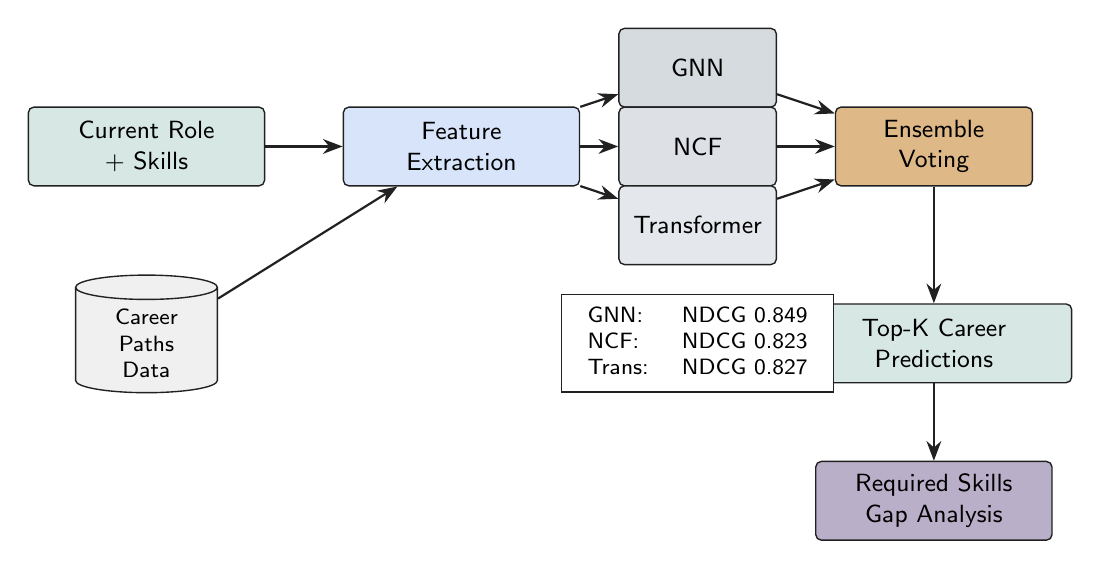
\begin{tikzpicture}[
    node distance=1.2cm,
    process/.style={rectangle, draw=textdark, rounded corners=2pt, fill=layer2!25, minimum width=3cm, minimum height=1cm, align=center, font=\small\sffamily, line width=0.5pt},
    data/.style={cylinder, draw=textdark, fill=databg, shape border rotate=90, aspect=0.3, minimum height=1.2cm, minimum width=1.8cm, align=center, font=\footnotesize\sffamily, line width=0.5pt},
    arrow/.style={-{Stealth[length=2.5mm]}, thick, color=textdark},
]

% Input
\node[process, fill=accentteal!30] (input) at (-5, 5) {Current Role\\+ Skills};

% Data sources
\node[data] (careerdata) at (-5, 2.5) {Career\\Paths\\Data};

% Feature extraction
\node[process] (features) at (-1, 5) {Feature\\Extraction};

% Models (parallel)
\node[process, fill=layer3!30, minimum width=2cm] (gnn) at (2, 6) {GNN};
\node[process, fill=layer3!25, minimum width=2cm] (ncf) at (2, 5) {NCF};
\node[process, fill=layer3!20, minimum width=2cm] (trans) at (2, 4) {Transformer};

% Ensemble
\node[process, fill=denseorange, minimum width=2.5cm] (ensemble) at (5, 5) {Ensemble\\Voting};

% Output
\node[process, fill=accentteal!30, minimum width=3.5cm] (output) at (5, 2.5) {Top-K Career\\Predictions};

% Skill gap
\node[process, fill=outputpurple, minimum width=3cm] (skillgap) at (5, 0.5) {Required Skills\\Gap Analysis};

% Arrows
\draw[arrow] (input) -- (features);
\draw[arrow] (careerdata) -- (features);
\draw[arrow] (features) -- (gnn);
\draw[arrow] (features) -- (ncf);
\draw[arrow] (features) -- (trans);
\draw[arrow] (gnn) -- (ensemble);
\draw[arrow] (ncf) -- (ensemble);
\draw[arrow] (trans) -- (ensemble);
\draw[arrow] (ensemble) -- (output);
\draw[arrow] (output) -- (skillgap);

% Metrics
\node[rectangle, draw=textdark, fill=white, font=\footnotesize\sffamily, line width=0.5pt] at (2, 2.5) {
\begin{tabular}{ll}
GNN: & NDCG 0.849\\
NCF: & NDCG 0.823\\
Trans: & NDCG 0.827
\end{tabular}
};

\end{tikzpicture}
\end{document}
